\documentclass[10pt,a4paper]{article}
\usepackage[T1]{fontenc}
\usepackage{lmodern,microtype,amsmath,amssymb,graphicx,booktabs,tabularx,array,longtable,xcolor,fancyhdr,titlesec}
\usepackage[margin=19mm,headheight=15pt,bottom=21mm]{geometry}
\usepackage[hidelinks,pdfauthor={},pdftitle={Current Architecture Three Stage TEC Cooled HgCdTe Assessment}]{hyperref}
\pdfinfoomitdate=1\pdftrailerid{}\pdfsuppressptexinfo=15
\definecolor{navy}{HTML}{19334B}\definecolor{blue}{HTML}{3E7099}\definecolor{rust}{HTML}{A35437}
\hypersetup{colorlinks=true,linkcolor=navy,urlcolor=blue}
\pagestyle{fancy}\fancyhf{}\fancyhead[L]{\scriptsize CURRENT-ARCHITECTURE ENGINEERING ASSESSMENT}\fancyhead[R]{\scriptsize 08 NOV 2026}
\fancyfoot[L]{\scriptsize Synthetic reference; not OEM-validated}\fancyfoot[R]{\scriptsize\thepage}
\setlength{\parindent}{0pt}\setlength{\parskip}{4pt}\setlength{\tabcolsep}{4pt}\renewcommand{\arraystretch}{1.12}
\setcounter{tocdepth}{1}
\titleformat{\section}{\Large\bfseries\color{navy}}{\thesection}{.55em}{}
\newcommand{\fig}[4][.91]{\begin{figure}[!htbp]\centering\includegraphics[width=#1\linewidth]{figures/#2.#3}\caption{#4}\end{figure}}
% Frozen source-derived tables. Auto-generated; do not hand-edit.
\newcommand{\stagebudgetrows}{1 & 58 & 179.9602 & 614.7396 & 1.086948 & 262.732 \\
2 & 22 & 46.1636 & 176.5165 & 0.325882 & 81.390 \\
3 & 8 & 5.1576 & 43.7058 & 0.096371 & 24.642 \\}
\newcommand{\cavityrows}{Ceramic C1 & 1.15901 & 0.20874 & 1.36775 \\
Ceramic C2 & 1.44533 & 0.23389 & 1.67923 \\
Ceramic C3 & 1.06469 & 0.15770 & 1.22239 \\
Detector & 0.22352 & 0.02375 & 0.24726 \\
TOTAL & 3.89255 & 0.62408 & 4.51663 \\}
\newcommand{\operatingrows}{Detector temperature (K) & 209.987981 & 210.625214 \\
Terminal voltage (V) & 1.524071 & 1.522462 \\
Electrical input (W) & 0.609628 & 0.608985 \\
Bath rejection (W) & 0.590323 & 0.594044 \\
Pressure (Pa) & 0 (cavity off) & 100 (Kr) \\}
\newcommand{\nodetablerows}{Stage0 Hot & 303.65655 \\
Stage0 Cold & 265.90329 \\
Stage1 Hot & 266.34287 \\
Stage1 Cold & 236.00259 \\
Stage2 Hot & 236.15716 \\
Stage2 Cold & 210.52765 \\
Carrier & 210.55066 \\
Die & 210.62521 \\}
\newcommand{\iterationrows}{1 & 210.599377 & 1.690e-02 & 3.914e-15 \\
2 & 210.624173 & 2.066e-03 & 4.580e-16 \\
3 & 210.625110 & 4.135e-04 & 1.478e-15 \\
4 & 210.625220 & 8.254e-05 & 2.928e-15 \\
5 & 210.625214 & 1.653e-05 & 5.503e-15 \\}
\newcommand{\residualrows}{Global energy & 8.8674e-09 & W \\
Worst stage balance & 4.9061e-09 & W \\
Ceramic pad heat & 5.5025e-15 & W \\
Worst individual leg & 1.2364e-13 & W \\
Final pad temperature change & 1.6535e-05 & K \\}
\newcommand{\materialrows}{40 & 31.477086 & 1.226120 & 2.776424 & -39.762194 & 0.837035 & 3.928920 \\
60 & 44.991486 & 1.550968 & 2.488935 & -53.616397 & 1.156199 & 3.246955 \\
80 & 60.679339 & 1.955036 & 2.260290 & -67.469437 & 1.522950 & 2.816874 \\
100 & 77.996604 & 2.446265 & 2.072406 & -81.936140 & 1.920207 & 2.536709 \\
120 & 96.944423 & 3.004830 & 1.909416 & -95.992742 & 2.354830 & 2.310364 \\
140 & 115.755946 & 3.567364 & 1.764537 & -109.847998 & 2.820018 & 2.129254 \\
160 & 133.684757 & 4.343818 & 1.630978 & -122.547039 & 3.319204 & 1.973635 \\
180 & 150.458980 & 5.175731 & 1.515526 & -134.499967 & 3.835302 & 1.851971 \\
200 & 166.078757 & 6.067058 & 1.415926 & -145.840430 & 4.371811 & 1.744414 \\
220 & 179.321421 & 7.073284 & 1.332165 & -156.231255 & 4.932113 & 1.653884 \\
240 & 190.594863 & 8.138932 & 1.257469 & -165.737958 & 5.570441 & 1.574639 \\
260 & 199.219885 & 9.351143 & 1.194083 & -174.568277 & 6.232621 & 1.506729 \\
280 & 205.739245 & 10.694094 & 1.137484 & -182.445326 & 6.884545 & 1.447332 \\
300 & 212.462550 & 12.080611 & 1.099006 & -189.575244 & 7.543277 & 1.399227 \\}
\newcommand{\legrows}{0 & 0 & N & -2.030000 & -2.030000 \\
1 & 0 & P & -1.450000 & -2.030000 \\
2 & 0 & N & -0.870000 & -2.030000 \\
3 & 0 & P & -0.290000 & -2.030000 \\
4 & 0 & N & 0.290000 & -2.030000 \\
5 & 0 & P & 0.870000 & -2.030000 \\
6 & 0 & N & 1.450000 & -2.030000 \\
7 & 0 & P & 2.030000 & -2.030000 \\
8 & 0 & N & 2.030000 & -1.450000 \\
9 & 0 & P & 1.450000 & -1.450000 \\
10 & 0 & N & 0.870000 & -1.450000 \\
11 & 0 & P & 0.290000 & -1.450000 \\
12 & 0 & N & -0.290000 & -1.450000 \\
13 & 0 & P & -0.870000 & -1.450000 \\
14 & 0 & N & -1.450000 & -1.450000 \\
15 & 0 & P & -2.030000 & -1.450000 \\
16 & 0 & N & -2.030000 & -0.870000 \\
17 & 0 & P & -1.450000 & -0.870000 \\
18 & 0 & N & -0.870000 & -0.870000 \\
19 & 0 & P & -0.290000 & -0.870000 \\
20 & 0 & N & 0.290000 & -0.870000 \\
21 & 0 & P & 0.870000 & -0.870000 \\
22 & 0 & N & 1.450000 & -0.870000 \\
23 & 0 & P & 2.030000 & -0.870000 \\
24 & 0 & N & 2.030000 & -0.290000 \\
25 & 0 & P & 1.450000 & -0.290000 \\
26 & 0 & N & 0.870000 & -0.290000 \\
27 & 0 & P & 0.290000 & -0.290000 \\
28 & 0 & N & -0.290000 & -0.290000 \\
29 & 0 & P & -0.870000 & -0.290000 \\
30 & 0 & N & -1.450000 & -0.290000 \\
31 & 0 & P & -2.030000 & -0.290000 \\
32 & 0 & N & -2.030000 & 0.290000 \\
33 & 0 & P & -1.450000 & 0.290000 \\
34 & 0 & N & -0.870000 & 0.290000 \\
35 & 0 & P & -0.290000 & 0.290000 \\
36 & 0 & N & 0.290000 & 0.290000 \\
37 & 0 & P & 0.870000 & 0.290000 \\
38 & 0 & N & 1.450000 & 0.290000 \\
39 & 0 & P & 2.030000 & 0.290000 \\
40 & 0 & N & 2.030000 & 0.870000 \\
41 & 0 & P & 1.450000 & 0.870000 \\
42 & 0 & N & 0.870000 & 0.870000 \\
43 & 0 & P & 0.290000 & 0.870000 \\
44 & 0 & N & -0.290000 & 0.870000 \\
45 & 0 & P & -0.870000 & 0.870000 \\
46 & 0 & N & -1.450000 & 0.870000 \\
47 & 0 & P & -2.030000 & 0.870000 \\
48 & 0 & N & -2.030000 & 1.450000 \\
49 & 0 & P & -1.450000 & 1.450000 \\
50 & 0 & N & -0.870000 & 1.450000 \\
51 & 0 & P & -0.290000 & 1.450000 \\
52 & 0 & N & 0.290000 & 1.450000 \\
53 & 0 & P & 0.870000 & 1.450000 \\
54 & 0 & N & 1.450000 & 1.450000 \\
55 & 0 & P & 2.030000 & 1.450000 \\
56 & 0 & N & 2.030000 & 2.030000 \\
57 & 0 & P & 1.450000 & 2.030000 \\
58 & 1 & N & 1.450000 & 0.870000 \\
59 & 1 & P & 0.870000 & 0.870000 \\
60 & 1 & N & 0.290000 & 0.870000 \\
61 & 1 & P & -0.290000 & 0.870000 \\
62 & 1 & N & -0.870000 & 0.870000 \\
63 & 1 & P & -1.450000 & 0.870000 \\
64 & 1 & N & -1.450000 & 0.290000 \\
65 & 1 & P & -0.870000 & 0.290000 \\
66 & 1 & N & -0.290000 & 0.290000 \\
67 & 1 & P & 0.290000 & 0.290000 \\
68 & 1 & N & 0.870000 & 0.290000 \\
69 & 1 & P & 1.450000 & 0.290000 \\
70 & 1 & N & 1.450000 & -0.290000 \\
71 & 1 & P & 0.870000 & -0.290000 \\
72 & 1 & N & 0.290000 & -0.290000 \\
73 & 1 & P & -0.290000 & -0.290000 \\
74 & 1 & N & -0.870000 & -0.290000 \\
75 & 1 & P & -1.450000 & -0.290000 \\
76 & 1 & N & -1.450000 & -0.870000 \\
77 & 1 & P & -0.870000 & -0.870000 \\
78 & 1 & N & -0.290000 & -0.870000 \\
79 & 1 & P & 0.290000 & -0.870000 \\
80 & 2 & N & 0.870000 & -0.290000 \\
81 & 2 & P & 0.290000 & -0.290000 \\
82 & 2 & N & -0.290000 & -0.290000 \\
83 & 2 & P & -0.870000 & -0.290000 \\
84 & 2 & N & -0.870000 & 0.290000 \\
85 & 2 & P & -0.290000 & 0.290000 \\
86 & 2 & N & 0.290000 & 0.290000 \\
87 & 2 & P & 0.870000 & 0.290000 \\}
\newcommand{\padrows}{0 & 6 & 0.000000 & 0.000000 & 1.584250 & 37.21000000 & -5.9404375264e-01 \\
0 & 8 & -2.030000 & -2.415000 & 2.084250 & 0.58100000 & +6.9212449542e-03 \\
0 & 9 & -1.160000 & -2.030000 & 2.084250 & 0.54000000 & +2.1001118011e-02 \\
0 & 10 & -0.000000 & -2.030000 & 2.084250 & 0.54000000 & +2.0799385661e-02 \\
0 & 11 & -2.030000 & -1.160000 & 2.084250 & 0.54000000 & +2.1333430585e-02 \\
0 & 12 & -1.160000 & -1.450000 & 2.084250 & 0.54000000 & +2.0925106301e-02 \\
0 & 13 & -1.160000 & -0.870000 & 2.084250 & 0.54000000 & +2.1098181465e-02 \\
0 & 14 & -2.030000 & -0.000000 & 2.084250 & 0.54000000 & +2.1661444954e-02 \\
0 & 15 & -1.160000 & -0.290000 & 2.084250 & 0.54000000 & +2.1280527762e-02 \\
0 & 16 & -0.000000 & -1.450000 & 2.084250 & 0.54000000 & +2.0726535211e-02 \\
0 & 17 & 0.000000 & -0.870000 & 2.084250 & 0.54000000 & +2.0872339885e-02 \\
0 & 18 & -0.000000 & -0.290000 & 2.084250 & 0.54000000 & +2.1135046258e-02 \\
0 & 19 & 1.160000 & -2.030000 & 2.084250 & 0.54000000 & +2.0762274895e-02 \\
0 & 20 & 2.030000 & -1.740000 & 2.084250 & 0.54000000 & +2.0894962316e-02 \\
0 & 21 & 1.160000 & -1.450000 & 2.084250 & 0.54000000 & +2.0664089207e-02 \\
0 & 22 & 1.160000 & -0.870000 & 2.084250 & 0.54000000 & +2.0730610371e-02 \\
0 & 23 & 1.160000 & -0.290000 & 2.084250 & 0.54000000 & +2.0987932670e-02 \\
0 & 24 & 2.030000 & -0.580000 & 2.084250 & 0.54000000 & +2.1025501033e-02 \\
0 & 25 & -1.160000 & 0.290000 & 2.084250 & 0.54000000 & +2.1501510390e-02 \\
0 & 26 & -2.030000 & 1.160000 & 2.084250 & 0.54000000 & +2.2056807823e-02 \\
0 & 27 & -1.160000 & 0.870000 & 2.084250 & 0.54000000 & +2.1665224003e-02 \\
0 & 28 & -1.160000 & 1.450000 & 2.084250 & 0.54000000 & +2.1972015528e-02 \\
0 & 29 & 0.000000 & 0.290000 & 2.084250 & 0.54000000 & +2.1329922044e-02 \\
0 & 30 & -0.000000 & 0.870000 & 2.084250 & 0.54000000 & +2.1513476612e-02 \\
0 & 31 & 0.000000 & 1.450000 & 2.084250 & 0.54000000 & +2.1762448001e-02 \\
0 & 32 & 1.160000 & 0.290000 & 2.084250 & 0.54000000 & +2.1132384800e-02 \\
0 & 33 & 2.030000 & 0.580000 & 2.084250 & 0.54000000 & +2.1315494607e-02 \\
0 & 34 & 1.160000 & 0.870000 & 2.084250 & 0.54000000 & +2.1316483722e-02 \\
0 & 35 & 1.160000 & 1.450000 & 2.084250 & 0.54000000 & +2.1497446937e-02 \\
0 & 36 & 0.088570 & 2.858995 & 2.084250 & 0.67225000 & -2.2200926469e-02 \\
0 & 37 & 2.030000 & 1.740000 & 2.084250 & 0.54000000 & +2.1652376653e-02 \\
0 & 38 & 1.450000 & 2.379622 & 2.084250 & 0.51850000 & +1.4709356454e-02 \\
1 & 44 & -1.740000 & -2.030000 & 2.684250 & 0.54000000 & -6.1717204457e-03 \\
1 & 45 & -0.580000 & -2.030000 & 2.684250 & 0.54000000 & -5.7923394592e-03 \\
1 & 46 & 0.580000 & -2.030000 & 2.684250 & 0.54000000 & -5.6313481447e-03 \\
1 & 47 & -1.740000 & -1.450000 & 2.684250 & 0.54000000 & -5.8945158835e-03 \\
1 & 48 & -1.740000 & -0.870000 & 2.684250 & 0.54000000 & -6.1272498337e-03 \\
1 & 49 & -0.580000 & -1.450000 & 2.684250 & 0.54000000 & -5.6677985879e-03 \\
1 & 50 & -0.580000 & -0.870000 & 2.684250 & 0.54000000 & -5.9073535857e-03 \\
1 & 51 & -1.740000 & -0.290000 & 2.684250 & 0.54000000 & -6.2861601984e-03 \\
1 & 52 & -1.740000 & 0.290000 & 2.684250 & 0.54000000 & -6.4929448577e-03 \\
1 & 53 & -0.580000 & -0.290000 & 2.684250 & 0.54000000 & -6.1441766581e-03 \\
1 & 54 & 0.580000 & -1.450000 & 2.684250 & 0.54000000 & -5.4949366062e-03 \\
1 & 55 & 0.580000 & -0.870000 & 2.684250 & 0.54000000 & -5.6165637076e-03 \\
1 & 56 & 0.580000 & -0.290000 & 2.684250 & 0.54000000 & -5.9284010470e-03 \\
1 & 57 & 1.740000 & -2.030000 & 2.684250 & 0.54000000 & -5.5964450493e-03 \\
1 & 58 & 1.740000 & -1.450000 & 2.684250 & 0.54000000 & -5.5750930796e-03 \\
1 & 59 & 1.740000 & -0.870000 & 2.684250 & 0.54000000 & -5.5316729855e-03 \\
1 & 60 & 1.740000 & -0.290000 & 2.684250 & 0.54000000 & -5.7862099653e-03 \\
1 & 61 & -0.580000 & 0.290000 & 2.684250 & 0.54000000 & -6.4257386885e-03 \\
1 & 62 & -1.740000 & 0.870000 & 2.684250 & 0.54000000 & -6.8576261766e-03 \\
1 & 63 & -1.740000 & 1.450000 & 2.684250 & 0.54000000 & -7.0890067759e-03 \\
1 & 64 & -0.580000 & 0.870000 & 2.684250 & 0.54000000 & -6.6249732312e-03 \\
1 & 65 & -0.580000 & 1.450000 & 2.684250 & 0.54000000 & -7.0137372522e-03 \\
1 & 66 & 0.580000 & 0.290000 & 2.684250 & 0.54000000 & -6.1746390641e-03 \\
1 & 67 & 0.580000 & 0.870000 & 2.684250 & 0.54000000 & -6.3948651910e-03 \\
1 & 68 & 0.580000 & 1.450000 & 2.684250 & 0.54000000 & -6.7126784447e-03 \\
1 & 69 & 1.740000 & 0.290000 & 2.684250 & 0.54000000 & -6.0016216656e-03 \\
1 & 70 & 1.740000 & 0.870000 & 2.684250 & 0.54000000 & -6.1198269805e-03 \\
1 & 71 & 1.740000 & 1.450000 & 2.684250 & 0.54000000 & -6.5247521871e-03 \\
1 & 72 & 1.740000 & 2.030000 & 2.684250 & 0.54000000 & -6.8707555753e-03 \\
1 & 74 & 0.870000 & 2.300000 & 3.184250 & 0.12000000 & +2.3941388903e-05 \\
1 & 75 & 1.450000 & 1.470862 & 3.184250 & 0.67900000 & +5.1504788556e-03 \\
1 & 76 & -1.450000 & -0.580000 & 3.184250 & 0.54000000 & +1.6210670281e-02 \\
1 & 77 & -0.580000 & -0.870000 & 3.184250 & 0.54000000 & +1.6207954022e-02 \\
1 & 78 & -0.580000 & -0.290000 & 3.184250 & 0.54000000 & +1.6071664242e-02 \\
1 & 79 & 0.290000 & -1.435162 & 3.184250 & 0.65650000 & +1.1539642240e-02 \\
1 & 80 & 0.580000 & -0.290000 & 3.184250 & 0.54000000 & +1.6217492734e-02 \\
1 & 81 & 1.450000 & 0.000000 & 3.184250 & 0.54000000 & +1.6376311378e-02 \\
1 & 82 & -1.450000 & 0.580000 & 3.184250 & 0.54000000 & +1.6153119097e-02 \\
1 & 83 & -0.580000 & 0.290000 & 3.184250 & 0.54000000 & +1.6048683270e-02 \\
1 & 84 & -0.580000 & 0.870000 & 3.184250 & 0.54000000 & +1.6098735692e-02 \\
1 & 85 & 0.580000 & 0.290000 & 3.184250 & 0.54000000 & +1.6138044094e-02 \\
1 & 86 & 0.580000 & 0.870000 & 3.184250 & 0.54000000 & +1.6218414034e-02 \\
2 & 92 & -1.160000 & -0.870000 & 3.784250 & 0.54000000 & -4.1229763184e-03 \\
2 & 93 & -1.160000 & -0.290000 & 3.784250 & 0.54000000 & -4.0325885849e-03 \\
2 & 94 & 0.000000 & -0.870000 & 3.784250 & 0.54000000 & -4.3372223253e-03 \\
2 & 95 & -0.000000 & -0.290000 & 3.784250 & 0.54000000 & -4.1255544021e-03 \\
2 & 96 & 1.160000 & -0.290000 & 3.784250 & 0.54000000 & -4.2477066490e-03 \\
2 & 97 & -1.160000 & 0.290000 & 3.784250 & 0.54000000 & -3.9991911145e-03 \\
2 & 98 & -1.160000 & 0.870000 & 3.784250 & 0.54000000 & -4.0132490723e-03 \\
2 & 99 & 0.000000 & 0.290000 & 3.784250 & 0.54000000 & -4.0452781812e-03 \\
2 & 100 & 1.160000 & 0.290000 & 3.784250 & 0.54000000 & -4.1617896577e-03 \\
2 & 101 & -0.000000 & 0.870000 & 3.784250 & 0.54000000 & -4.1215621922e-03 \\
2 & 102 & 1.160000 & 0.870000 & 3.784250 & 0.54000000 & -4.3855401752e-03 \\
2 & 104 & 0.870000 & 0.829062 & 4.284250 & 0.64000000 & +8.5720985048e-03 \\
2 & 105 & 0.692720 & -0.929413 & 4.284250 & 0.81350000 & +3.2580848072e-03 \\
2 & 106 & -0.000000 & -0.290000 & 4.284250 & 0.54000000 & +1.1238504436e-02 \\
2 & 107 & -0.870000 & 0.000000 & 4.284250 & 0.54000000 & +1.1290111066e-02 \\
2 & 108 & 0.000000 & 0.290000 & 4.284250 & 0.54000000 & +1.1233859859e-02 \\
3 & 114 & 0.580000 & 0.290000 & 4.884250 & 0.54000000 & -1.2327805666e-03 \\
3 & 115 & -0.580000 & -0.290000 & 4.884250 & 0.54000000 & -1.2229792254e-03 \\
3 & 116 & 0.580000 & -0.290000 & 4.884250 & 0.54000000 & -1.2662612022e-03 \\
3 & 117 & -0.580000 & 0.290000 & 4.884250 & 0.54000000 & -1.2279447029e-03 \\
3 & 119 & -0.000000 & -0.000000 & 5.384250 & 4.41000000 & +4.9499656971e-03 \\}

\newcommand{\legrowsA}{0 & 0 & N & -2.030000 & -2.030000 \\
1 & 0 & P & -1.450000 & -2.030000 \\
2 & 0 & N & -0.870000 & -2.030000 \\
3 & 0 & P & -0.290000 & -2.030000 \\
4 & 0 & N & 0.290000 & -2.030000 \\
5 & 0 & P & 0.870000 & -2.030000 \\
6 & 0 & N & 1.450000 & -2.030000 \\
7 & 0 & P & 2.030000 & -2.030000 \\
8 & 0 & N & 2.030000 & -1.450000 \\
9 & 0 & P & 1.450000 & -1.450000 \\
10 & 0 & N & 0.870000 & -1.450000 \\
11 & 0 & P & 0.290000 & -1.450000 \\
12 & 0 & N & -0.290000 & -1.450000 \\
13 & 0 & P & -0.870000 & -1.450000 \\
14 & 0 & N & -1.450000 & -1.450000 \\
15 & 0 & P & -2.030000 & -1.450000 \\
16 & 0 & N & -2.030000 & -0.870000 \\
17 & 0 & P & -1.450000 & -0.870000 \\
18 & 0 & N & -0.870000 & -0.870000 \\
19 & 0 & P & -0.290000 & -0.870000 \\
20 & 0 & N & 0.290000 & -0.870000 \\
21 & 0 & P & 0.870000 & -0.870000 \\
22 & 0 & N & 1.450000 & -0.870000 \\
23 & 0 & P & 2.030000 & -0.870000 \\
24 & 0 & N & 2.030000 & -0.290000 \\
25 & 0 & P & 1.450000 & -0.290000 \\
26 & 0 & N & 0.870000 & -0.290000 \\
27 & 0 & P & 0.290000 & -0.290000 \\
28 & 0 & N & -0.290000 & -0.290000 \\
29 & 0 & P & -0.870000 & -0.290000 \\
30 & 0 & N & -1.450000 & -0.290000 \\
31 & 0 & P & -2.030000 & -0.290000 \\
32 & 0 & N & -2.030000 & 0.290000 \\
33 & 0 & P & -1.450000 & 0.290000 \\
34 & 0 & N & -0.870000 & 0.290000 \\
35 & 0 & P & -0.290000 & 0.290000 \\
36 & 0 & N & 0.290000 & 0.290000 \\
37 & 0 & P & 0.870000 & 0.290000 \\
38 & 0 & N & 1.450000 & 0.290000 \\
39 & 0 & P & 2.030000 & 0.290000 \\
40 & 0 & N & 2.030000 & 0.870000 \\
41 & 0 & P & 1.450000 & 0.870000 \\
42 & 0 & N & 0.870000 & 0.870000 \\
43 & 0 & P & 0.290000 & 0.870000 \\}
\newcommand{\legrowsB}{44 & 0 & N & -0.290000 & 0.870000 \\
45 & 0 & P & -0.870000 & 0.870000 \\
46 & 0 & N & -1.450000 & 0.870000 \\
47 & 0 & P & -2.030000 & 0.870000 \\
48 & 0 & N & -2.030000 & 1.450000 \\
49 & 0 & P & -1.450000 & 1.450000 \\
50 & 0 & N & -0.870000 & 1.450000 \\
51 & 0 & P & -0.290000 & 1.450000 \\
52 & 0 & N & 0.290000 & 1.450000 \\
53 & 0 & P & 0.870000 & 1.450000 \\
54 & 0 & N & 1.450000 & 1.450000 \\
55 & 0 & P & 2.030000 & 1.450000 \\
56 & 0 & N & 2.030000 & 2.030000 \\
57 & 0 & P & 1.450000 & 2.030000 \\
58 & 1 & N & 1.450000 & 0.870000 \\
59 & 1 & P & 0.870000 & 0.870000 \\
60 & 1 & N & 0.290000 & 0.870000 \\
61 & 1 & P & -0.290000 & 0.870000 \\
62 & 1 & N & -0.870000 & 0.870000 \\
63 & 1 & P & -1.450000 & 0.870000 \\
64 & 1 & N & -1.450000 & 0.290000 \\
65 & 1 & P & -0.870000 & 0.290000 \\
66 & 1 & N & -0.290000 & 0.290000 \\
67 & 1 & P & 0.290000 & 0.290000 \\
68 & 1 & N & 0.870000 & 0.290000 \\
69 & 1 & P & 1.450000 & 0.290000 \\
70 & 1 & N & 1.450000 & -0.290000 \\
71 & 1 & P & 0.870000 & -0.290000 \\
72 & 1 & N & 0.290000 & -0.290000 \\
73 & 1 & P & -0.290000 & -0.290000 \\
74 & 1 & N & -0.870000 & -0.290000 \\
75 & 1 & P & -1.450000 & -0.290000 \\
76 & 1 & N & -1.450000 & -0.870000 \\
77 & 1 & P & -0.870000 & -0.870000 \\
78 & 1 & N & -0.290000 & -0.870000 \\
79 & 1 & P & 0.290000 & -0.870000 \\
80 & 2 & N & 0.870000 & -0.290000 \\
81 & 2 & P & 0.290000 & -0.290000 \\
82 & 2 & N & -0.290000 & -0.290000 \\
83 & 2 & P & -0.870000 & -0.290000 \\
84 & 2 & N & -0.870000 & 0.290000 \\
85 & 2 & P & -0.290000 & 0.290000 \\
86 & 2 & N & 0.290000 & 0.290000 \\
87 & 2 & P & 0.870000 & 0.290000 \\}

\newcommand{\legpairrows}{0 & 0 & N & -2.030000 & -2.030000 & 44 & 0 & N & -0.290000 & 0.870000 \\
1 & 0 & P & -1.450000 & -2.030000 & 45 & 0 & P & -0.870000 & 0.870000 \\
2 & 0 & N & -0.870000 & -2.030000 & 46 & 0 & N & -1.450000 & 0.870000 \\
3 & 0 & P & -0.290000 & -2.030000 & 47 & 0 & P & -2.030000 & 0.870000 \\
4 & 0 & N & 0.290000 & -2.030000 & 48 & 0 & N & -2.030000 & 1.450000 \\
5 & 0 & P & 0.870000 & -2.030000 & 49 & 0 & P & -1.450000 & 1.450000 \\
6 & 0 & N & 1.450000 & -2.030000 & 50 & 0 & N & -0.870000 & 1.450000 \\
7 & 0 & P & 2.030000 & -2.030000 & 51 & 0 & P & -0.290000 & 1.450000 \\
8 & 0 & N & 2.030000 & -1.450000 & 52 & 0 & N & 0.290000 & 1.450000 \\
9 & 0 & P & 1.450000 & -1.450000 & 53 & 0 & P & 0.870000 & 1.450000 \\
10 & 0 & N & 0.870000 & -1.450000 & 54 & 0 & N & 1.450000 & 1.450000 \\
11 & 0 & P & 0.290000 & -1.450000 & 55 & 0 & P & 2.030000 & 1.450000 \\
12 & 0 & N & -0.290000 & -1.450000 & 56 & 0 & N & 2.030000 & 2.030000 \\
13 & 0 & P & -0.870000 & -1.450000 & 57 & 0 & P & 1.450000 & 2.030000 \\
14 & 0 & N & -1.450000 & -1.450000 & 58 & 1 & N & 1.450000 & 0.870000 \\
15 & 0 & P & -2.030000 & -1.450000 & 59 & 1 & P & 0.870000 & 0.870000 \\
16 & 0 & N & -2.030000 & -0.870000 & 60 & 1 & N & 0.290000 & 0.870000 \\
17 & 0 & P & -1.450000 & -0.870000 & 61 & 1 & P & -0.290000 & 0.870000 \\
18 & 0 & N & -0.870000 & -0.870000 & 62 & 1 & N & -0.870000 & 0.870000 \\
19 & 0 & P & -0.290000 & -0.870000 & 63 & 1 & P & -1.450000 & 0.870000 \\
20 & 0 & N & 0.290000 & -0.870000 & 64 & 1 & N & -1.450000 & 0.290000 \\
21 & 0 & P & 0.870000 & -0.870000 & 65 & 1 & P & -0.870000 & 0.290000 \\
22 & 0 & N & 1.450000 & -0.870000 & 66 & 1 & N & -0.290000 & 0.290000 \\
23 & 0 & P & 2.030000 & -0.870000 & 67 & 1 & P & 0.290000 & 0.290000 \\
24 & 0 & N & 2.030000 & -0.290000 & 68 & 1 & N & 0.870000 & 0.290000 \\
25 & 0 & P & 1.450000 & -0.290000 & 69 & 1 & P & 1.450000 & 0.290000 \\
26 & 0 & N & 0.870000 & -0.290000 & 70 & 1 & N & 1.450000 & -0.290000 \\
27 & 0 & P & 0.290000 & -0.290000 & 71 & 1 & P & 0.870000 & -0.290000 \\
28 & 0 & N & -0.290000 & -0.290000 & 72 & 1 & N & 0.290000 & -0.290000 \\
29 & 0 & P & -0.870000 & -0.290000 & 73 & 1 & P & -0.290000 & -0.290000 \\
30 & 0 & N & -1.450000 & -0.290000 & 74 & 1 & N & -0.870000 & -0.290000 \\
31 & 0 & P & -2.030000 & -0.290000 & 75 & 1 & P & -1.450000 & -0.290000 \\
32 & 0 & N & -2.030000 & 0.290000 & 76 & 1 & N & -1.450000 & -0.870000 \\
33 & 0 & P & -1.450000 & 0.290000 & 77 & 1 & P & -0.870000 & -0.870000 \\
34 & 0 & N & -0.870000 & 0.290000 & 78 & 1 & N & -0.290000 & -0.870000 \\
35 & 0 & P & -0.290000 & 0.290000 & 79 & 1 & P & 0.290000 & -0.870000 \\
36 & 0 & N & 0.290000 & 0.290000 & 80 & 2 & N & 0.870000 & -0.290000 \\
37 & 0 & P & 0.870000 & 0.290000 & 81 & 2 & P & 0.290000 & -0.290000 \\
38 & 0 & N & 1.450000 & 0.290000 & 82 & 2 & N & -0.290000 & -0.290000 \\
39 & 0 & P & 2.030000 & 0.290000 & 83 & 2 & P & -0.870000 & -0.290000 \\
40 & 0 & N & 2.030000 & 0.870000 & 84 & 2 & N & -0.870000 & 0.290000 \\
41 & 0 & P & 1.450000 & 0.870000 & 85 & 2 & P & -0.290000 & 0.290000 \\
42 & 0 & N & 0.870000 & 0.870000 & 86 & 2 & N & 0.290000 & 0.290000 \\
43 & 0 & P & 0.290000 & 0.870000 & 87 & 2 & P & 0.870000 & 0.290000 \\}

\begin{document}
\thispagestyle{empty}\vspace*{6mm}
{\color{navy}\rule{\linewidth}{1.5pt}}
\vspace{8mm}
{\Huge\bfseries\color{navy} Three-Stage TEC-Cooled\\[2mm] HgCdTe Detector\par}
\vspace{7mm}{\LARGE Current Architecture and Engineering Assessment\par}
\vspace{8mm}{\large Synthetic 824-solid replacement cooler / 88-leg hybrid simulation / 8 November 2026\par}
\vspace{5mm}
\noindent\fbox{\begin{minipage}{.96\linewidth}\small
\textbf{CONDITIONAL TECHNICAL ASSESSMENT.} This is a separate current-architecture document. The historical 38-page Revision 3 report describes an older 216-domain cooler; its scientific methods remain useful, but its internal copper geometry is not the present design. The 43-page interim edition is preserved independently.
\end{minipage}}
\vspace{4mm}
\begin{center}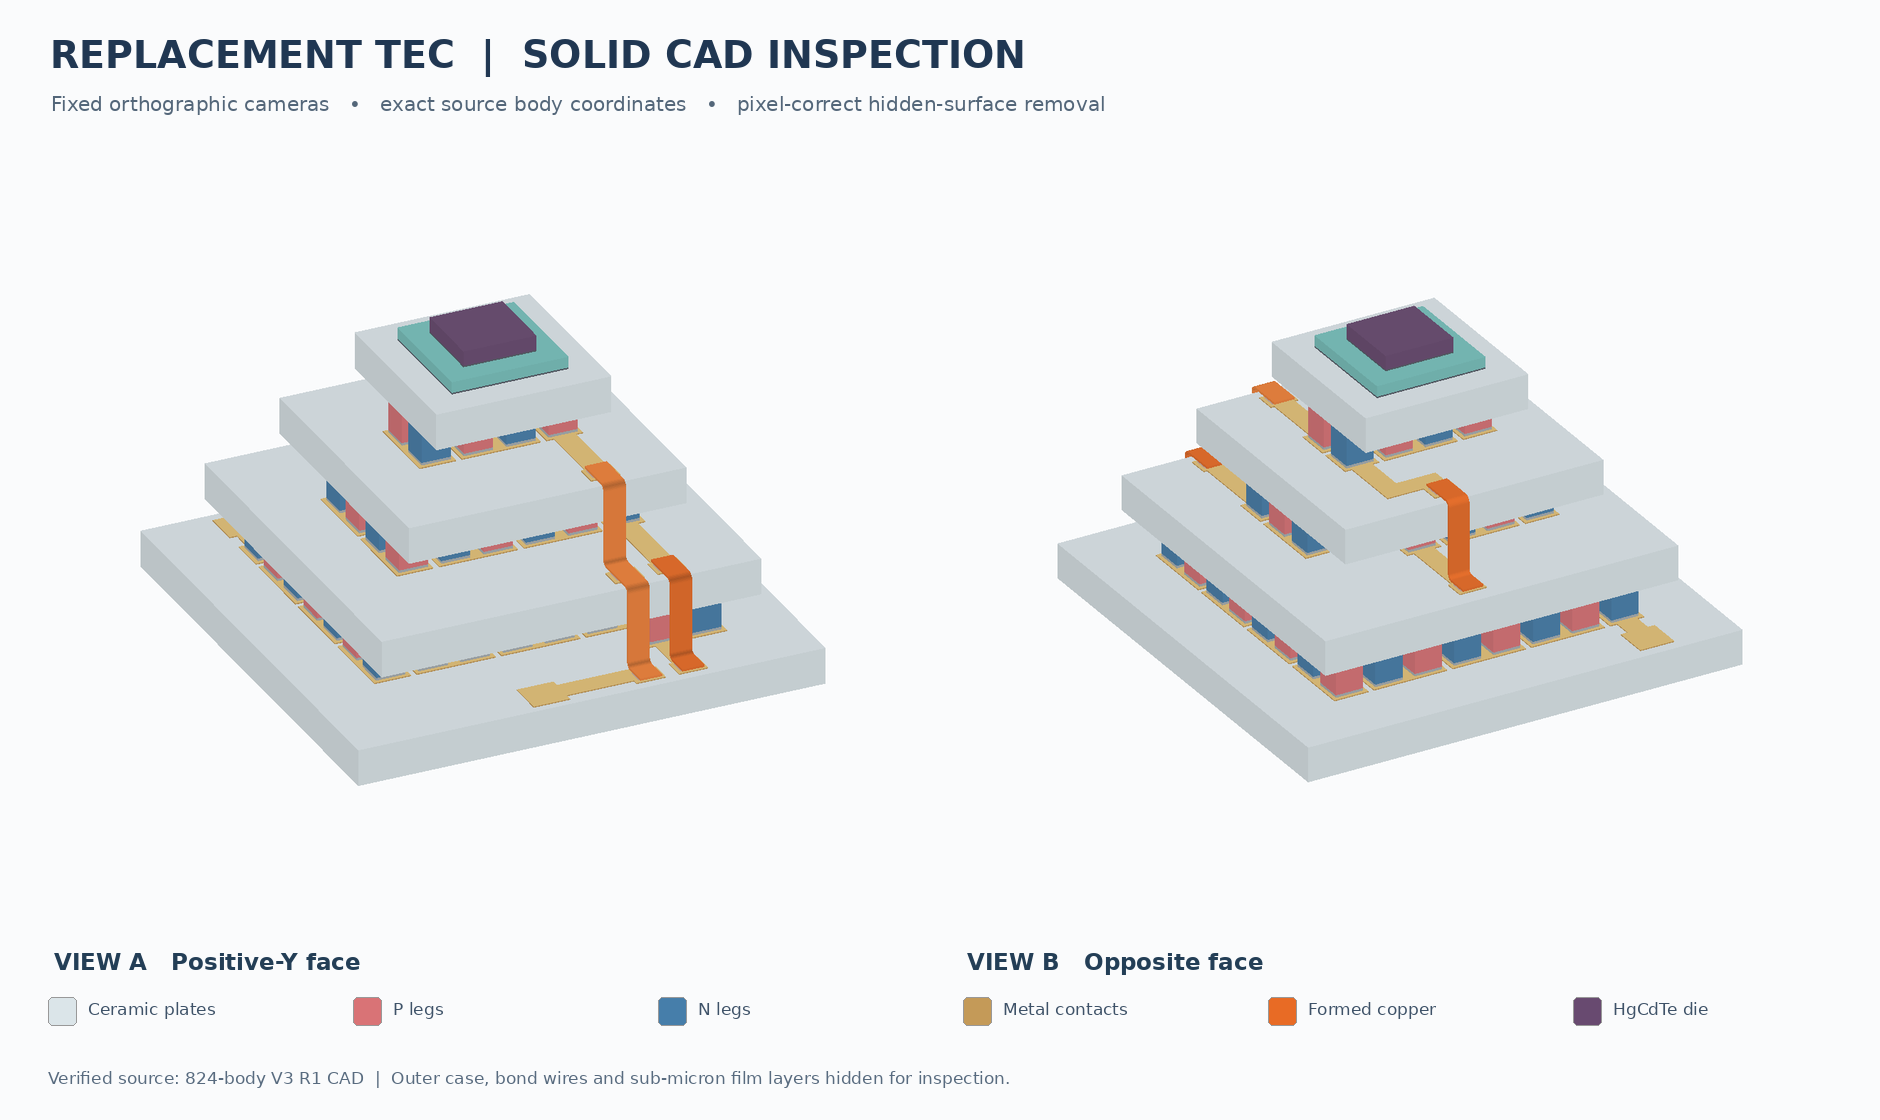
\includegraphics[width=.97\linewidth]{figures/tec_solid_inspection.png}\end{center}
\vspace{3mm}
{\small Shaded opaque display of the original frozen V3 replacement CAD body primitives and analytical formed-tab bends. The enclosure, external leads and micron-scale layers are hidden for inspection. This remains geometry evidence, not a fully coupled 430-domain PDE or a manufactured device.}
\vfill
{\color{navy}\rule{\linewidth}{1pt}}
{\small\textbf{Reading contract.} All measured/source-backed quantities, selected synthetic construction assumptions, computed numerical outputs and outstanding validation failures are explicitly distinguished.}
\clearpage
\section*{Executive technical abstract}\addcontentsline{toc}{section}{Executive technical abstract}
The modeled article is a plausible but synthetic three-stage thermoelectrically cooled HgCdTe photoconductor in a nine-pin TO-66-style package. Its redesigned physical cooler comprises 824 STEP solids; its derived 430-domain geometry has 2,440 native face regions. It contains 88 series P/N legs (29/11/4 couples) plus short formed interstage tabs and a three-foot stepped return. Independent CAD review supports conditional constructibility, not demonstrated manufacture or reliable electrical/thermal operation.

The current functioning V3.3 solver represents each leg by 32 nonlinear axial transport intervals and resolves four original 3D ceramic P1 FEM fields with 11,791 tetrahedra, plus assumed solder/contact losses, Cu/Au external leads, detector thermal load, hot mounting, effective krypton and gray radiation. For a 0.400 A, 300 K, 2 mW detector, 100 Pa Kr case, it gives
\[
\boxed{T_{\rm die}=210.625214\ \mathrm{K}},\quad
\boxed{V_{\rm term}=1.522462\ \mathrm{V}},\quad
\boxed{P_{\rm in}=0.608985\ \mathrm{W}}.
\]
The cavity contributes 4.516629 mW into the cold components, with a numerically closed global energy residual of approximately \(8.8674\times10^{-9}\) W.

\textbf{Critical architectural limitation.} The formed interstage copper tab and multi-level return geometry has a verified circuit topology, but its nonlocal metal current, contact and thermal-shunt effects have \emph{not} yet been fully included as a coupled 3D electrothermal field operator in V3.3. The nominal detector temperature is thus conditional on an important unresolved physical coupling. The complete 430-domain PDE has not been run and its global candidate mesh has substantial poor-quality regions.

This assessment retains actual CAD renderings, true ceramic fields, equations, transport profiles, full 88-leg/pad numerical boundary records, and explicit verification statistics. The older 38-page Rev3 is retained as a separate historical benchmark, rather than being confused with the current cooler.
\clearpage
\tableofcontents\clearpage
\section{Version identity and evidence hierarchy}
\begin{tabularx}{\linewidth}{p{30mm}p{37mm}X}\toprule
Artifact & Subject & Verified status\\\midrule
Historical Rev3 & Earlier 216-solid 28/12/4 cooler & Detailed field method; raw-gradient release failed\\
Replacement V3 R1 & 824 physical STEP bodies, formed tabs and joints & Conditional CAD design acceptance\\
R3.9 geometry & 430 material regions, 2,440 CAD faces & Geometric mesh audit; conditioning unqualified\\
V3.3 simulation & 88 nonlinear legs and four source 3D ceramic fields & One accepted numerical operating point; interstage metal physics incomplete\\\bottomrule\end{tabularx}

The cooler envelope is informed by TEC Microsystems MC04 family reference geometry; the package by a separate VIGO nine-pin TO-66 drawing. They are not identified as a commercially fabricated composite. The 29/11/4 stage split, material grades, solder properties and fabricated metal details are source-inspired or chosen synthetic hypotheses, \emph{not} proprietary OEM internals.
\section{Replacement TEC physical architecture}
Four nominal ceramic plates have square footprints 6.4, 5.2, 3.8 and 2.4 mm, each 0.5 mm thick. Eighty-eight P/N legs are 0.4 by 0.4 by 0.5 mm each, grouped into 58, 22 and 8 legs from hot to cold. The package routing connects TEC supply/return pins 1/9 and separate HgCdTe photoconductor bias pins 7/8. The exported reference contains 824 CAD solids and 176 solder joints, 89 insulated TEC electrical nets, and formed internal metal links.
\fig[.94]{cad_package}{png}{Genuine archived V3 replacement STEP package rendering. The package and cooler geometry are independently selected engineering references, not the geometry of one identified manufactured product.}
The original long, unsupported copper routing was rejected. The replacement has formed Cu-family foil tabs across nets 58 and 80, plus an extended three-foot return net 88 with a real middle thermal landing. Its design uses patterned ceramic metallization and finite solder footprints. The selected foil section is 0.300 by 0.030 mm; its bend radius is 0.075 mm; finished foot joints are specified at 20 plus/minus 5 micrometres. No measured current rating or fatigue qualification follows.
\fig[.84]{cad_interfaces}{png}{Actual CAD-derived joint, metallization and mounting sections. Joining tolerances and material/process choices remain selected synthetic requirements.}
\clearpage

\section{Shaded solid CAD inspection: the actual replacement geometry}
The shaded views below tessellate the original 824-body source geometry using a true per-pixel depth buffer. The previous mean-face-depth renderer wrongly displayed hidden metallization through ceramic solids. This rendering is neither a reconstructed cooler nor an exploded assembly. All plates, P/N legs and analytically bent copper foil links retain the source positions, widths, heights, polarities and original path radii. Compared with the wireframe, the opaque solid bodies make the differences from the rejected long copper-post construction readily visible.

\fig[.98]{tec_solid_inspection}{png}{Correctly depth-occluded replacement geometry from two orthographic views: four ceramic stages, 58/22/8 P/N legs, visible exposed metallization only, and actual formed copper-foil connections. The external case, leads and very thin buried film layers are intentionally omitted. Original analytic foil-bend paths are sampled for shaded display, without relocating any CAD features.}
\clearpage
\subsection{Actual interstage foil cross-sections}
The design uses two short supported formed copper-foil stage links (nets 58 and 80), and a longer stepped return (net 88). The last has two vertical steps and three physical feet, including an intermediate thermal landing. Unlike a generic connecting rod, its cross-section has nominal width 0.300 mm, thickness 0.030 mm and bend radius 0.075 mm. The foil is represented at actual thickness, not enlarged for visibility.

\fig[.98]{tec_formed_tab_sections}{png}{Y--Z sections reconstructed from the source analytic straight and circular-arc geometry at original coordinates, without exploded offsets. Pale blue regions indicate where ceramic cross-sections intersect each foil plane. The 30-micrometre copper thickness is drawn at true scale.}
This inspection demonstrates the geometry change, but does not resolve missing formed-tab Joule heating, interface thermal resistance, electrothermal current crowding or interstage thermal bypass. Those remain necessary before the V3.3 detector-temperature estimate can qualify as a prediction for the assembled design.
\clearpage

\section{Series topology and copper parasitics}
The CAD conductor graph verifies all 88 legs as articulation vertices in the pin-1-to-pin-9 series circuit: removing any one leg disconnects the two terminals. Native transitions pass from P leg 57 to N leg 58 through tab 58, and from P79 to N80 through tab 80. The final leg P87 is connected to pin 9 through stepped return 88. These checks prove intended topology but not the temperature-dependent electrical or thermal properties of the connections.
\fig[.92]{v33_topology}{pdf}{Actual saved stage-specific P/N leg centroids and plate footprints. This verifies the source positions used in the working hybrid; it does not depict a solved copper-tab thermal field.}
For a uniform slender conductor with temperature-dependent material properties,
\[
 R_e=\int_0^L{\rho(T,s)\over A(s)}\,ds,\qquad
 G_{\rm th}=\left[\int_0^L{ds\over k(T,s)A(s)}\right]^{-1},\quad
 P_J=I^2 R_e.
\]
The registered neutral path lengths are 1.96062 mm (net58), 1.97062 mm (net80), and 3.70624 mm (return88). Using a uniform 0.300 by 0.030 mm section, illustrative \(\rho_{\rm Cu}=1/(58\times10^6)\,\Omega{\rm m}\) and \(k_{\rm Cu}=385\,\mathrm{W/(m\,K)}\) yields the approximate geometry-only screen below.
\fig[.92]{tab_screen}{pdf}{Derived idealized uniform-bar electrical and thermal copper coefficients. Actual formed-tab bends, patterned multilayer film, contact drops, variable temperatures, Joule partition and intermediate return landing are not resolved. The return is not correctly represented by a single two-terminal thermal conductance.}
The competing design goals are explicit: reducing electrical resistance through a larger cross-section raises passive thermal coupling. A physical successor must solve or independently validate the full nonlocal stage-to-stage multiport heat and current network, including the return's intermediate land.

\section{Global geometric and meshing milestones}
The first full R3.8 TetGen volume candidate contained 1,043,314 tetrahedra over 430 material regions, with all 320,522 registered facets and 378 finite-contact witnesses retained. R3.9 applied 33,195 conservative 3-to-2 internal connectivity operations and reduced the mesh to 1,010,119 tetrahedra with unchanged original surface facets and regional volumes.
\fig[.91]{mesh_quality}{pdf}{Independent archived global mesh-quality measurements. The 3-to-2 flips improved the poor-cell population, but the minimum quality and remaining weak cells prevent assuming mesh-converged coupled FEM.}
R3.9 retains 241,754 tetrahedra with mean-ratio quality below 0.05 (23.93 percent) and a minimum of \(1.38495\times10^{-4}\). Thus no global coupled 430-domain electrical and thermal PDE is released. Historical full-solid electrical Gate B is FAIL/STOP; the first source N/P pair had eight raw gradient-current failures; the prospective P2 and global C/D computations are not qualified. Good energy closure in a separate hybrid model does not erase these original raw gates.

\section{Governing nonlinear thermoelectric model}
Each of the 88 axial P/N legs uses a signed 0.4 A series current and 32 longitudinal intervals. With \(z\) directed hot-to-cold, \(S(T)\) Seebeck coefficient, \(\rho(T)\) resistivity, \(k(T)\) conductivity, and signed current density \(J\), the constitutive conservation model is
\[
q=S(T)TJ-k(T){dT\over dz},\qquad
{dq\over dz}=J\left[\rho(T)J+S(T){dT\over dz}\right],\qquad
{dV\over dz}=\rho(T)J+S(T){dT\over dz}.
\]
Midpoint constitutive evaluation and damped Newton iterations enforce thermal and electrical conservation at local temperatures, including the boundary identity \(Q_h-Q_c=IV_{\mathrm{leg}}\). The material source is a 14-knot figure digitization of research P-HE and N-HE-1 specimens over 40--300 K. Above 300 K the code uses an \emph{unmeasured} one-quarter final-segment slope continuation; this is not a production material characterization.
\fig[.92]{v33_transport}{pdf}{Source-derived P/N research analog properties. The shaded/dashed extension beyond 300 K is explicitly assumed; 58 hot-stage leg contacts exceed the research marker range.}

\section{Original three-dimensional ceramic FEM}
Each ceramic independently solves
\[
-\nabla\cdot(k_c\nabla T)=0,\qquad
K_{ab}=\sum_e\int_{\Omega_e}k_c\nabla N_a\cdot\nabla N_b\,d\Omega,\quad
b_a=\sum_f\int_{A_f}N_a q_f\,dA,
\]
with \(k_c=30\,\mathrm{W/(m\,K)}\) a selected constant-property alumina analogue. Original face-specific P/N leg heat and assumed joint/cavity contributions are distributed over native TRI3 pad faces; source-local pad means feed back into leg end temperatures. Four archived source meshes contain 4,936 / 4,085 / 1,986 / 784 TET4 elements, totaling 11,791 tetrahedra.
\fig[.96]{v33_ceramic_fields}{pdf}{Real source-tetrahedron top-surface triangulations and solved nodal temperature fields from the original saved four ceramic archives. This is authentic spatial FEM evidence rather than a rendered approximation of the uncomputed full global package.}
The four fields share their temperature gauge and stage heat exchange with the nonlocal reduced network. This is a single-mesh spatial result; no independent mesh-converged thermal accuracy bound is available.
\clearpage
\section{Solder, lead and contact accounting}
The current synthetic electrical model assumes 176 solder bodies of 35 micrometres thickness and 0.16 mm$^2$ area, with assumed SnSb resistivity \(1.7\times10^{-7}\ \Omega\,{\rm m}\) and 352 assumed metal-interface specific resistances \(r_c^{\prime\prime}=10^{-11}\ \Omega\,{\rm m}^2\). For each joint the resistance is
\[
R_j=\rho_{\rm SnSb}{L_j\over A_j}+2{r_c^{\prime\prime}\over A_j},\quad
R_{\rm all}=0.028545\ \Omega,\quad I^2R_{\rm all}=4.56720\ {\rm mW}.
\]
The implementation places 25.950 micowatts per source joint into its neighboring ceramic pad. This assumes the entire joint Joule heat reaches a ceramic and omits finite thermal-contact drops, interfacial thermopower and nonlocal copper-network heating. The four ceramic applied-joint terms, in mW, are [1.50510, 2.07600, 0.77850, 0.20760].
External supply Cu wires and detector Au bonds are separate effective electrical/thermal links. \emph{They must not be mistaken for a resolved calculation of the newly formed tabs or return conductor.}

\section{Cavity and hot-side boundary assumptions}
The reference forward case imposes a 300 K cap/window/ambient thermal reservoir, a 100 Pa krypton environment, an effective 3.0 mm gas gap, accommodation 0.8, and nominal gas conductivity knots \(k_{\rm Kr}(200,300,400\,{\rm K})=(0.0064,0.0095,0.0122)\ {\rm W/(m\,K)}\).
Gray radiation uses assumed emissivities \(\epsilon_{\rm cap}=0.20\), \(\epsilon_{\rm ceramic}=0.80\), and \(\epsilon_{\rm window}=0.10\), with selected effective view factors. The source effective exposed surface areas are [12.60, 8.68, 4.76, 1.00] mm$^2$. The generic exchange terms are
\[
Q_{{\rm gas},i}=G_{\rm eff,i}(p,T)(T_\infty-T_i),\qquad
Q_{{\rm rad},i}=\epsilon_{{\rm eff},i}\sigma A_iF_i(T_\infty^4-T_i^4).
\]
These are \emph{effective engineering closures}, not cavity fluid dynamics, true free-molecular transport, exact exposed-face loads, spectral window modeling or full radiosity.
\fig[.92]{v33_cavity_loads}{pdf}{Archived V3.3 cavity contributions: total gas 3.892553 mW, gray radiation 0.624076 mW, combined heat into cold components 4.516629 mW. The reservoir carries an equal and opposite signed load.}
\begin{center}\small\begin{tabular}{lrrr}\toprule
Cold destination & Kr gas (mW) & Gray rad. (mW) & Total (mW)\\\midrule
\cavityrows
\bottomrule\end{tabular}\end{center}
An effective header/TIM/radiator resistance of approximately 4.8334 K/W carries heat to the warm sink. Neither mount pressure nor material lot is an experimental datum. The cavity load is redistributed to native \emph{upper metal-pad} sources in the current model; thermal gradients on exposed bare ceramic faces are not thereby demonstrated.

\section{Matched current reference cases}
The V3.2 baseline and V3.3 cavity-loaded run use the same 88-leg source geometry, 11,791 ceramic tetrahedra, 0.4 A input, 300 K reservoir, 2 mW detector load and assumed material/contact parameters. The cavity raises die temperature \(0.637233\) K, while the nonlinear terminal voltage changes slightly due to changed operating gradients.
\begin{center}\small\begin{tabular}{lrr}\toprule
Metric & V3.2 (cavity off) & V3.3 (cavity on)\\\midrule
\operatingrows
\bottomrule\end{tabular}\end{center}
\fig[.92]{v33_versions}{pdf}{Recorded V1 to V3.3 complete reference-model milestones, all evaluated at the nominal current. These points describe changing model fidelity, not successive mesh convergence or independent measurements.}

\section{Stage heat, voltage and temperature results}
\begin{center}\small\begin{tabular}{rrrrrr}\toprule
Stage & Legs & Cold flux (mW) & Hot flux (mW) & V & Joule (mW)\\\midrule
\stagebudgetrows
\bottomrule\end{tabular}\end{center}
\begin{center}\small\begin{tabular}{lr}\toprule Coupled node & Temperature (K)\\\midrule
\nodetablerows
\bottomrule\end{tabular}\end{center}
The external terminal voltage includes additional lead and joint contributions beyond summed P/N voltage. Stage energies must account for signed electrical work, source losses, detector heat, cavity sources and external sink. Directly adding cavity milliwatts to input electrical power without solving the changed stage temperatures would be incorrect.
\fig[.92]{v33_leg_budgets}{pdf}{Real saved individual-leg cold-side heat and terminal-voltage contributions. Stage transitions occur after source leg indices 57 and 79. Source material laws and local ceramic pad temperatures determine leg-specific behavior.}

\section{Fixed-point convergence and independent accounting}
The solver used the previous V3.2 solution as a warm start and iterated five spatial leg/pad updates, stopping at a maximum pad temperature change \(1.65345\times10^{-5}\) K below its registered \(2\times10^{-5}\) K criterion. That number is a \emph{numerical stopping threshold}, not a temperature accuracy bound.
\fig[.90]{v33_iterations}{pdf}{Actual saved spatial fixed-point iteration changes and detector temperature history. The last update meets the registered coarse convergence threshold; no mesh refinement or material uncertainty bound is inferred.}
\begin{center}\scriptsize\begin{tabular}{rrrr}\toprule
Iteration & Die T (K) & Max pad update (K) & Local flux mismatch (W)\\\midrule
\iterationrows
\bottomrule\end{tabular}\end{center}
\begin{center}\small\begin{tabular}{lrl}\toprule Metric & Absolute residual & Unit\\\midrule
\residualrows
\bottomrule\end{tabular}\end{center}
An independent read-only field/load audit reconstructs the saved energy terms without rerunning the original PDE and finds a finite \(2.535\times10^{-8}\) W pad/leg update discrepancy. Numerical closure validates the \emph{declared equations and discretization bookkeeping} at this operating point, not prediction fidelity of the as-built cooler.
\clearpage
\section{Engineering conclusion and next milestone}
The replacement cooler is a concrete 824-solid design with original STEP files, audited contact geometry and a stage-specific 430-region mesh. It is \emph{not} necessary to restart cooler CAD development. The functioning V3.3 hybrid omits full nonlocal electrothermal field solutions for its formed tab58/tab80/return88 conductors, so the conditional temperature prediction cannot yet be called a full electrothermal result for the physical replacement.
The next practical engineering milestone is a conservative electrical and thermal multiport extracted from this already constructed CAD, with named intermediate thermal landings and explicit film, solder and contact effects. The solver should then recompute the same 0.400 A / 300 K / 2 mW / 100 Pa nominal point and report changed die temperature, terminal voltage, stage heat budgets and sensitivity to uncertain contact inputs. Full 3D copper FEM may be justified if compact validated metal substructures cannot bound current crowding or nonlocal heat flow.
The older 38-page Revision 3 is preserved because of its unusually useful FEM methodology and publication-level plots, \emph{not} because it describes the current metal layout. The 43-page interim extension is historical, not the latest design reference.

\section{Independent scientific reproduction}
An independent implementation should use the four 0.5 mm-thick 6.4/5.2/3.8/2.4 mm ceramics, the Appendix B 88 leg centers and polarities, the 29/11/4-couple electrical series order and the source-selected 0.4 by 0.4 by 0.5 mm P/N geometry. Apply all six 14-knot P/N research-material curves in Appendix A; interpolate within the experimental range and explicitly impose the unmeasured quarter-final-segment-slope continuation above 300 K.
Solve 88 individually signed 32-interval nonlinear axial thermoelectric legs and four source-geometry P1 ceramic steady conduction systems using local native TRI3 heat-face integrals. Set the declared assumed ceramic conductivity to 30 W/(m K), add the nominal 176 SnSb joints and 352 assumed electrical contacts, Cu and Au external leads, 2 mW detector heat, the stated finite mounting resistance and the effective 100 Pa Kr/gray radiation closure. Iterate local pad and leg flux/temperature feedback until the maximum change is below 0.000020 K and independently check all signed stage and total heat balances.
The archived Appendix C face centroids, areas and flux totals permit a comparable heat-integral replication, not byte-exact nodal temperatures. Bitwise reproduction requires original tetrahedral connectivity, exact face polygon vertices, quadrature and solver conventions. No unpublished real-world detector measurements are claimed.
\section{Scientific and engineering references}
\begin{enumerate}
\item TEC Microsystems, three-stage 3MC04-044-05 cooler family datasheet (2019), external envelope and thermoelectric reference. Its hidden internal routing is unknown.
\item VIGO Photonics, 3TE TO-66 nine-pin housing reference, Rev. 9 (2024). The cooler and housing are independent reference products.
\item J. Zhang et al., low-temperature bismuth telluride thermoelectric measurement and error-analysis study, \emph{Chinese Physics Letters} 42, 056304 (2025). DOI \href{https://doi.org/10.1088/0256-307X/42/5/056304}{10.1088/0256-307X/42/5/056304}. Source P-HE and N-HE-1 specimens are not the actual installed module.
\item M. L. Huber, gas thermal conductivity tabulations (NIST/CRC, 2019): krypton material reference, not experimentally measured gap conduction.
\item TEC Microsystems and Kryotherm multistage construction drawings and photographs; Coherent mounting guidelines. These establish process families, not qualification of the selected synthetic formed-tab design.
\end{enumerate}
\clearpage
\appendix
\section{Complete 14-knot P and N transport source tables}
The following 84 values comprise six figure-digitized research-specimen curves. They do not establish actual commercial material properties. The assumed extension beyond 300 K is
\[
f(T)=f(300)+0.25\,(T-300)\frac{f(300)-f(280)}{20},
\qquad f\in\{S,\rho,k\}.
\]
{\scriptsize\setlength{\tabcolsep}{2.5pt}
\begin{center}\begin{tabular}{rrrrrrr}\toprule
\(T\) K & \(S_P\) & \(\rho_P\) & \(k_P\) & \(S_N\) & \(\rho_N\) & \(k_N\)\\
 & \(\mu{\rm V/K}\) & \(\mu\Omega\,{\rm m}\) & W/(m K) & \(\mu{\rm V/K}\) & \(\mu\Omega\,{\rm m}\) & W/(m K)\\\midrule
\materialrows
\bottomrule\end{tabular}\end{center}}
\clearpage
\section{All original 88 P/N leg centers}
Each leg has 0.1600 mm$^2$ area and 0.5000 mm axial length; stage index 0 is the hottest. All coordinates refer to the original selected synthetic CAD x/y frame in mm.
{\scriptsize\renewcommand{\arraystretch}{1.04}
\begin{longtable}{rrrrr}\toprule
Series index & Stage & P/N & \(x\) (mm) & \(y\) (mm)\\\midrule\endfirsthead
\toprule Series index & Stage & P/N & \(x\) (mm) & \(y\) (mm)\\\midrule\endhead
\legrows
\bottomrule\end{longtable}}
\clearpage
\section{Native ceramic-face geometric and solved heat ledger}
For each original ceramic and native thermal face, the table lists source face ID, centroid (mm), original CAD area (mm$^2$) and the signed integrated solved heat \emph{into} that ceramic (W). Contributions include local P/N transport, provisional joint heating, finite sink, detector and effective cavity loads when applicable. Exact face polygons are not fully specified by centroids and areas.
{\scriptsize\setlength{\tabcolsep}{2pt}\renewcommand{\arraystretch}{1.06}
\begin{longtable}{rrrrrrr}\toprule
Cer. & Face ID & \(x\) & \(y\) & \(z\) & Area mm$^2$ & Heat in (W)\\\midrule\endfirsthead
\toprule Cer. & Face ID & \(x\) & \(y\) & \(z\) & Area & Heat (W)\\\midrule\endhead
\padrows
\bottomrule\end{longtable}}
\clearpage
\section{Verification boundaries and remaining work}
\begin{tabularx}{\linewidth}{p{38mm}p{30mm}X}\toprule
Technical claim & Actual status & Appropriate requirement for improvement\\\midrule
824-solid replacement V3 CAD & Conditional physical-design PASS & Measured forming, solder, current and reliability capability\\
Native pin-to-pin topology & 88/88 legs PASS & Finite real current density, resistance and contact temperature fields\\
Global 430-domain R3.9 mesh & Geometric PASS & Improve worst elements and prove solver conditioning/convergence\\
Original full-solid electrical Gate B & Historical FAIL/STOP & Qualify original raw-gradient tests on a viable mesh\\
Full 430-domain electrothermal PDE & NOT RUN & Integrated metal/contact/leg/ceramic field solution\\
V3.3 hybrid at 0.4 A & Numerical PASS & Copper multiport closure, material sensitivity and current/load response\\
Rarefied gas and radiation & Effective load model & Native exposed-surface gas/gray/spectral physics\\
Real thermoelectric grades & Unidentified & Bounded synthetic studies or actual module certificates\\
HgCdTe photodetection & No carrier/optical PDE & Detector noise/spectral/bias physics if needed\\
As-built product prediction & Unvalidated & Device measurements; do not claim manufacturer equivalence\\\bottomrule
\end{tabularx}
\vspace{5mm}

{\color{navy}\rule{\linewidth}{1pt}}

{\small\textbf{Publication policy.} The original 38-page Revision 3 remains a sealed separate historical methodology reference. Its later 43-page interim source-mesh integration is likewise archived. This document describes the newer replacement CAD and the most recent completed running hybrid with the unmodeled internal copper paths prominently disclosed. All figures and numerical tables derive from existing saved evidence, and no new physics calculation was performed for this publication.}
\end{document}
